\section{Theorie}
\label{sec:Theorie}

\subsection{Faraday Effekt}
\label{subsec:faraday}
Unter dem Faraday Effekt versteht man die Drehung der Polarisationsebene eines
Lichtstrahls, der ein von einem Magnetfeld durchflussenes Medium durchquert.
Er tritt nur auf, wenn der Lichtstrahl linear polarisiert ist und das Magnetfeld
im Medium eine Komponente parallel zur Ausbreitungsrichtung des Strahl besitzt.

Dieser Effekt beruht darauf, dass die Phasengeschwindigkeiten im Medium für links- und
rechtszirkular polarisiertes Licht verschieden sind und sich eine linear polarisierte
Welle als aus einer links- und einer rechtszirkular polarisierten Welle zuasmmengesetzt
verstehen lässt. Er wird daher auch zirkulare Doppelbrechung genannt.

Im vom B-Feld durchflossenen Medium werden durch die Gitteratome und die Bandelektronen
Dipolmomente erzeugt, die zu einer Polarisation
\begin{equation}
  \vec{P} = \epsilon_0 \chi \vec{E}
  \label{eqn:polarisation}
\end{equation}
des Mediums führen. Dabei ist $\vec{P}$ die Polarisation, $\epsilon_0$ die
Dielektrizitätskonstante, $\chi$ die dielektrische Suszeptibilität und
$\vec{E}$ das elektrische Feld. In anisotropen Materialien wird $\chi$ zum Tensor.
Dieser hat (für einfache Fälle) die Form
\begin{align}
  \chi =
  \left( \begin{matrix}
         \chi_{\mathrm{xx}} & -i \chi_{\mathrm{xy}} & 0 \\
         -i \chi_{\mathrm{yx}} & \chi_{\mathrm{xx}} & 0 \\
         0 & 0 & \chi_{\mathrm{zz}}  \\
  \end{matrix} \right)\,.
  \label{eqn:chitensor}
\end{align}
Dabei sind die beiden Nichtdiagonalelemente komplex konjugiert zueinander. Wird das
Matrial nicht von einem B-Feld durchflossen, so ist es optisch inaktiv und der
Tensor besitzt nur Diagonalelemente:
\begin{align}
  \chi =
  \left( \begin{matrix}
         \chi_{\mathrm{xx}} & 0 & 0 \\
         0 & \chi_{\mathrm{xx}} & 0 \\
         0 & 0 & \chi_{\mathrm{zz}}  \\
  \end{matrix} \right) \,.
  \label{eqn:chitensor2}
\end{align}
Daran ist erkennbar, dass zunächst isotrope Materie zu anisotroper Materie wird,
wenn sie von einem B-Feld durchflossen wird.

Der Winkel, um den das Licht beim Durchlaufen des Mediums gedreht wird, lässt sich zu
\begin{align}
  \theta \approx \frac{L \omega}{2 c n}\chi_{\mathrm{xy}}
  \label{eqn:theta1}
\end{align}
nähern. Dabei ist $\theta$ der Drehwinkel, $L$ die Länge der Probe, $\omega$ die Frequenz
der Lichtwelle, $c$ die Vakuumlichtgeschwindigkeit, $n$ der Berchungsindex des Mediums
und $\chi_{\mathrm{xy}}$ ein Eintrag des $\chi$-Tensors.

Für sichtbares Licht kann der Rotationswinkel zu
\begin{align}
  \theta \approx \frac{e^3_0}{2 \epsilon_0 c} \frac{1}{m^2}\frac{\omega^2}{(\omega^2_0 - \omega^2)^2} \frac{NBL}{n}
  \label{eqn:theta2}
\end{align}
bestimmt werden. Dabei ist $e_0$ die Elektronladung, $m$ die Masse des Elektrons, $N$
die Anzahl an Elektronen pro Volumen und $\omega_0$ die Resonanzfrequenz.


\subsection{Bandstruktur von Festkörpern}
\label{subsec:bandstruktur}

Kristalle haben im Allgemeinen eine komplizierte Bandstruktur. Je nach Beschaffenheit
der Bandstruktur werden Metalle, Halbleiter und Isolatoren voneinander unterschieden.
Skizzen dazu befinden sich in Abbildung \ref{fig:bandstruktur}.
Bei Metallen ist das Leitungsband halb besetzt, was eine gute elektrische Leitfähigkeit
mit sich bringt. Bei Halbleitern befindet sich zwischen dem Leitungsband und dem
Valenzband eine kleine Bandlücke, die durch Energiezufuhr überwunden
werden kann, sodass Elektronen ins Leitungsband gelangen und das Material elektrisch
leitend wird. In Isolatoren ist diese Bandlücke so groß, dass sie praktisch nicht
überwunden werden kann und damit auch keine Elektronen ins Leitsungsband gelangen.

\begin{figure}[h!]
  \centering
  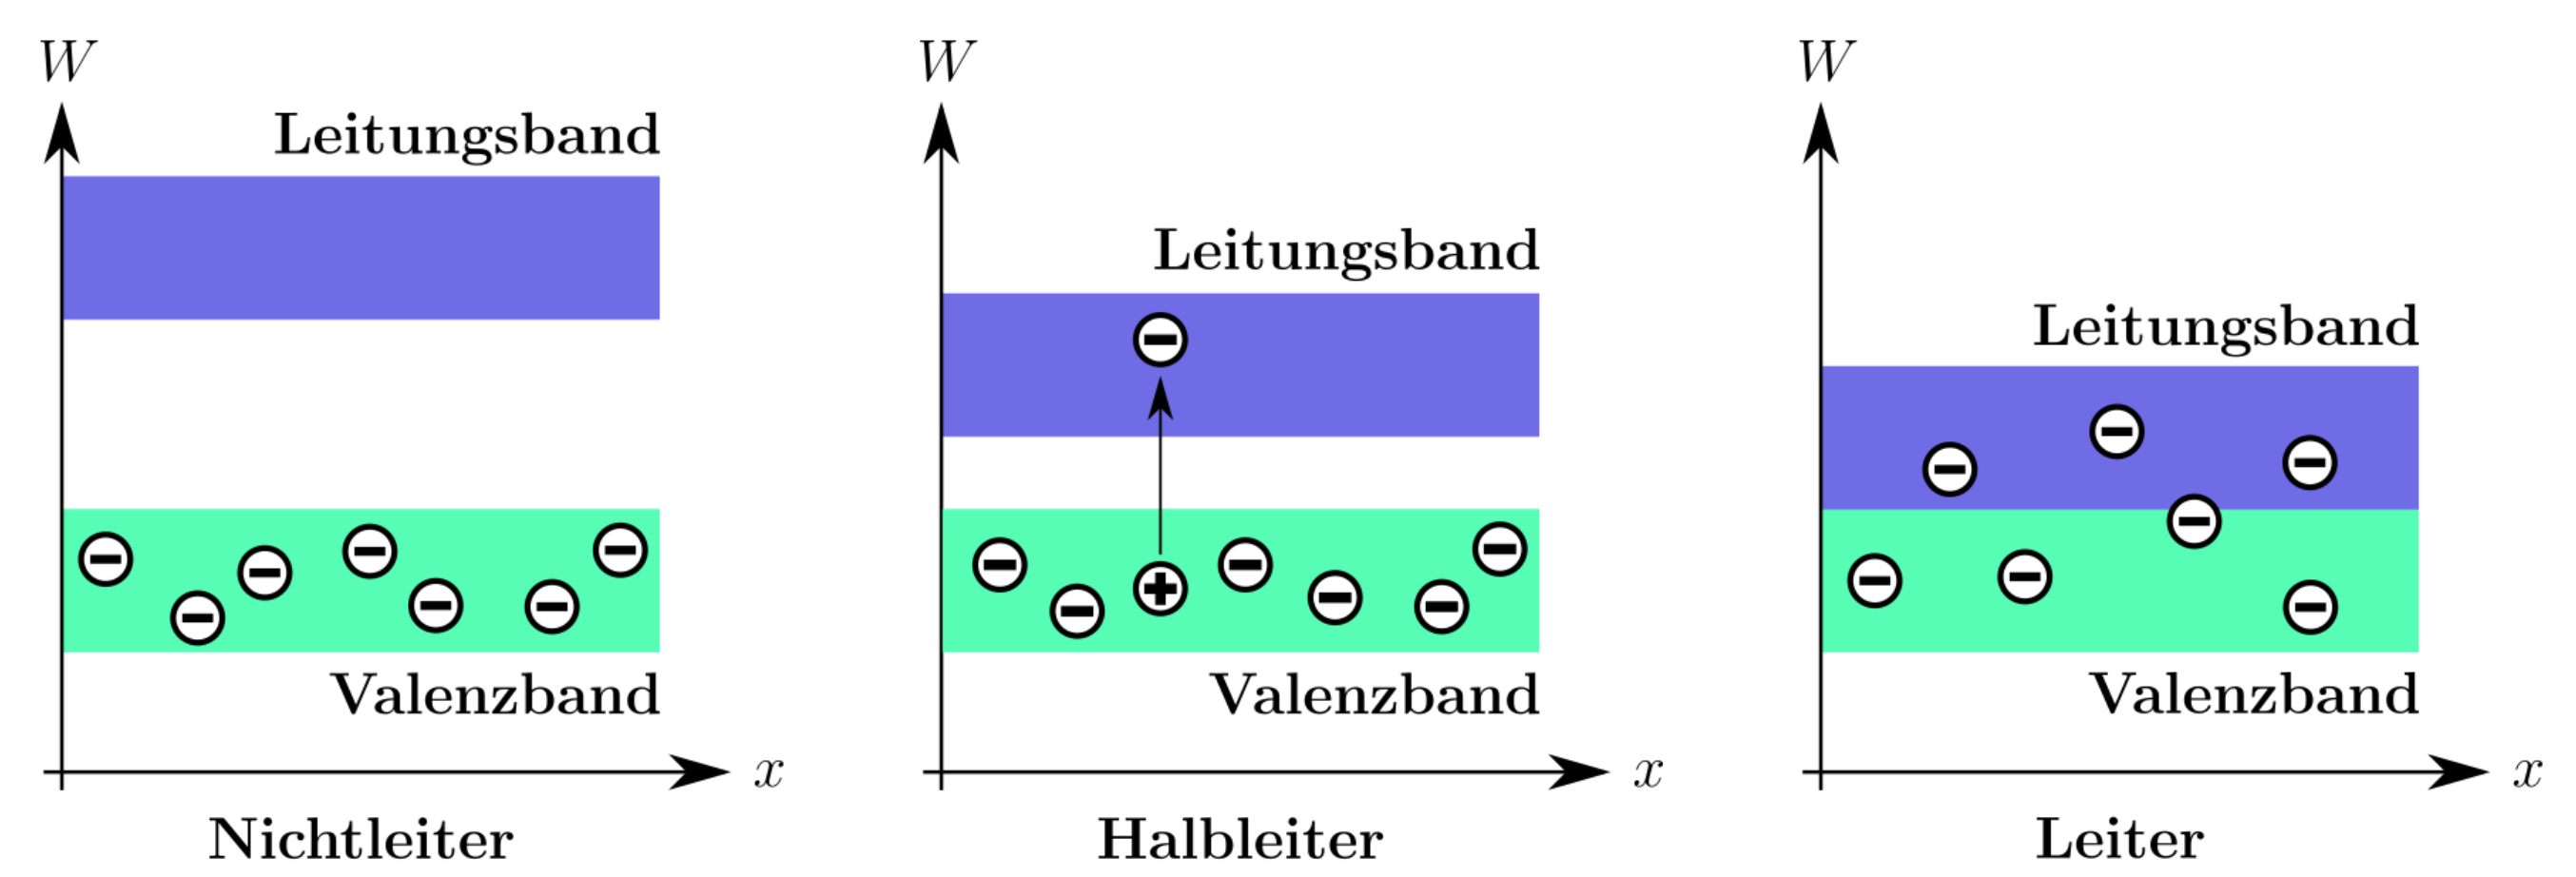
\includegraphics[width=\textwidth]{data/bandstruktur.png}
  \caption{Skizze der Bandstruktur für Metalle, Halbleiter und Isolatoren \cite{wiki}.}
  \label{fig:bandstruktur}
\end{figure}

\subsection{Dotierung von Halbleitern}
\label{subsec:dotierung}
Durch Dotierung kann die elektrische Leitfähigkeit eines Halbleiters beeinflusst werden.
Dabei werden Atome eines anderen Stoffes in das Gitter des Halbleiters gebracht.
Bei der n-Dotierung wird ein höherwertiges Element (Donator) ins Gitter gebracht, welches
dann ein Elektron abgeben kann, das sich daraufhin quasi frei im Gitter bewegen kann.
Dies entspricht im Bändermodell einem Elektron nahe dem Leitungsband, welches leicht
ins dieses angehoben werden kann. An der Stelle
des Donators entsteht eine ortsfeste positive Ladung.
Die p-Dotierung ist das Gegenstück zur n-Dotierung. Hier wird ein niedrigerwertiges
Element (Akzeptor) in das Gitter eingebracht. Da hier ein Elektron zu wenig vorliegt,
entsteht ein sog. Defektelektron, also ein Elektronenloch. Dieses verhält sich
wie eine positive Ladung. Im Bändermodell entspricht das einer Ladung
nahe dem Valenzband. An der Stelle
des Akzeptors bleibt eine ortsfeste negative Ladung zurück.

\subsection{Effektive Masse}
\label{subsec:effmass}
Die Bandstruktur von Festkörpern ist oft so kompliziert, dass es für einfache Berechnungen
einiger Approximationen bedarf. Für Halbleiter lässt sich die Bandkante des Leitungsbandes
näherungsweise beschreiben durch eine Funktion $\epsilon(\vec{k})$. Dabei ist
$\epsilon$ die Elektronenenergie und $\vec{k}$ der Wellenzahlvektor. Dies lässt sich
in eine Taylorreihe entwickeln:
\begin{align}
  \epsilon(k) = \epsilon (0) + \frac{1}{2} \sum_{i=1}^3 \left(\frac{\partial \epsilon^2}{\partial k^2_{\mathrm{i}}}\right)_{k=0} k_{\mathrm{i}}^2 + ... \,.
  \label{eqn:taylor}
\end{align}
Durch Vergleich mit der Beziehung
\begin{equation}
  \epsilon = \frac{\hbar^2 k^2}{2m}
  \label{eqn:elektronenergie}
\end{equation}
für die Elektronenenergie findet man
\begin{equation}
   m^*_{\mathrm{i}} := \frac{\hbar}{\left(\frac{\partial \epsilon^2}{\partial k^2_{\mathrm{i}}}\right)_{k=0}} \,.
   \label{eqn:effmass}
\end{equation}
Für sehr symmetrische Kristalle liegen kugelförmige Energieflächen vor. In diesem
Band können Elektronen dann betrachtet werden wie freie Teilchen. Dies kann auf
Gleichung \eqref{eqn:theta2} angewandt werden und man erhält
\begin{align}
  \theta_{\mathrm{frei}} = \frac{e^3_0}{8 \pi^2 \epsilon_0 c^3}\frac{1}{\left(m^{*}\right)^2} \lambda^2 \frac{NBL}{n} \,.
  \label{eqn:theta_frei}
\end{align}
$\theta_{\mathrm{frei}}$ ist als die Faraday-Rotation pro Einheitslänge zu verstehen und
$\lambda$ ist die Wellenlänge des Lichts. Es wurden alle Massen durch die effektiven
Massen ersetzt, was die Bestimmung der effektiven Masse der Elektronen mithilfe der
Faraday-Rotation ermöglicht. Es ist darauf hinzuweisen, dass dieser Zusammenhang nur
gültig ist, wenn die Elektronen als frei angenommen werden können, da nur in diesem
Fall $\omega_0 \rightarrow 0$ gilt.
